\documentclass[../main.tex]{subfiles}
%\graphicspath{{\subfix{images/}}}


\begin{document}

%\section{Learning with errors (LWE)}
\label{section:lwe}

% \kl{lwe has been used as the security base for many applications including public key encryption, HE, etc, see the 4th paragraph in \citep{lyubashevsky2010ideal}.}

In Section \ref{section:lattice theory}, we have introduced the SIS\index{SIS} problem, which is an average-case problem whose difficulty is based on the worst-case hardness of three lattice problems. The main drawback of SIS-based cryptosystems is the impractical public key size and ciphertext size. Typically, the key size is $\Tilde{O}(n^4)$ and the plaintext size is $\Tilde{O}(n^2)$, where $n$ is a security parameter with typical values in the hundreds. \footnote{$\Tilde{O}(\cdot)$ is a variation of the $O(\cdot)$ notation that ignores logarithmic terms: $\Tilde{O}(g(n))=O(g(n) \log^k n)$ for some $k$. This time complexity class is known as \textbf{quasilinear time} and sometimes expressed as $O(n^{1+\epsilon})$ for an $\epsilon >0$.}
% \kl{Remain of the SIS problem and give an example of a specific SIS-based cryptosysmte, so the readers can see the computational inefficiency.}

The \textbf{learning with error (LWE)}\index{LWE} problem was introduced by \citet{regev05} as another foundational problem for building lattice-based cryptosystems with provable security but smaller key and ciphertext size. 
% It allows one to build a cryptosystem with smaller key size and ciphertext size, while still retaining the same provable security from some worst-case lattice problems. 
In particular, LWE-based cryptosystems' public key size is $\Tilde{O}(n^2)$, which is a considerable improvement from SIS-based ones, although still not practical for large $n$. In addition, the plaintext size  is increased by only $\Tilde{O}(1)$ times once encrypted.  


Intuitively, the LWE problem tries to recover a secret key from a system of noisy linear equations. To draw an analogy, if the linear equations are not noisy, the problem can be solved efficiently using Gaussian elimination as shown in the following example. 

\begin{example}
Given three linear equations of the form $Ax=B$, where $A$ is a 3 by 3 matrix, $B$ is a 3 by 1 matrix and $x$ is a 1 by 3 matrix, we can use Gaussian elimination (a.k.a. row reduction) to turn $A$ into an upper triangular matrix, hence solving for the solution $x$. 
\begin{small}
\[
\left[
\begin{array}{ccc|c}
1 & 3 & 1 & 9  \\
1 & 1 & -1 & 1  \\
3 & 11 & 5 & 35  \\
\end{array}
\right]
\]    

\[
\left[
\begin{array}{ccc|c}
1 & 3 & 1 & 9  \\
0 & -2 & -2 & -8  \\
0 & 2 & 2 & 8  \\
\end{array}
\right]
\]    

\[
\left[
\begin{array}{ccc|c}
1 & 3 & 1 & 9  \\
0 & -2 & -2 & -8  \\
0 & 0 & 0 & 0  \\
\end{array}
\right]
\]

\[
\left[
\begin{array}{ccc|c}
1 & 0 & -2 & 3  \\
0 & 1 & 1 & 4  \\
0 & 0 & 0 & 0  \\
\end{array}
\right]
\]
\end{small}
\end{example}
\noindent The LWE problem, however, introduces noises (or errors) into the linear equations, making the above problem significantly harder. More precisely, Gaussian elimination involves linear combinations of rows. This process may amplify the noises so that the resulting rows are unable to maintain the original information that is embedded in the equations. 

\iffalse 
In LWE setting, $\chi$ is often assumed to concentrate on ``small integers''. That is, for small $\alpha \ll 1$,
\begin{equation*}
    Pr\left(\mathbf{x} \leftarrow \chi \mid ||\mathbf{x}|| > \alpha q\right) < negl(n),
\end{equation*}
where $negl(n)$ is a
\reversemarginpar
\marginnote{\textit{Negligible function}}
\textbf{negligible function}.\footnote{A function $\mu: \N \rightarrow \R$ is \textbf{negligible} if for every positive integer $c$, there exists an integer $N_c$ such that for all $x > N_c$, we have $|\mu(x)| < x ^{-c}$.} 
We use the \textbf{big-Theta} notation $f(n) = \Theta(g(n))$ to denote the asymptotic behaviour of the function $f(n)$ if there exists constants $c_1$, $c_2$ and $n_0$ such that for all $n > n_0$, the function is bounded between by $c_1 g(n) \le f(n) \le c_2 g(n)$. 
\fi 


%%%%%%%%%%%%%%%%%%%%%%%%%%%%%%%%%%%%%%%%%%%%%%%%%%%%%%%%%%%%%%%%%%%%%%%%%%%%%%%%%%%%%%%%%%%%%%%%%%%


\subsection{LWE distribution}
\label{subsec:lweDist}

We introduce and recall some notations before going into the main content of this section. Denote $\Z / q\Z$ by $\Z_q$ and let $\Z_q^n = \{( a_1, \dots, a_n) \mid a_i \in \Z_q\}$ be its $n$-dimensional generalization. 
The notation $\mathbf{x} \leftarrow \Z_q^n$ indicates $\mathbf{x}$ is uniformly sampled from $\Z_q^n$. 
Let $\T=\R/\Z=[0,1)$ be $\R \bmod 1$.

In regards to errors in the LWE samples, we use $\phi$ and $\chi$ to denote the error distributions over $\T$ and $\Z_q$, respectively. In the hardness proof, \cite{regev2009lattices} set the error distribution $\phi=\Psi_{\alpha}$ which can be obtained by sampling from a continuous Gaussian with mean 0 and standard deviation $\frac{\alpha}{\sqrt{2\pi}}$ (or scale $\alpha$) and reducing the outputs modulo 1. But in practice, these errors are discretized for convenience by multiplying samples from $\Psi_{\alpha}$ by $q$ and rounding to the nearest integer modulo $q$. This gives rise to the discretized error distribution $\Bar{\Psi}_{\alpha}$ over $\Z_q$. 

Throughout his work, \citep{regev2009lattices} proved the hardness result of LWE based on the continuous error distribution $\Psi_{\alpha}$ and only used the discretized error $\Bar{\Psi}_{\alpha}$ when presenting a secure LWE-based cryptosystem. In fact, both error distributions entail the same hardness of the LWE problem as emphasized by Lemma 4.3 in \citep{regev2009lattices}. For simplicity, we present the LWE problem and its hardness proof based on the discretized error distribution $\chi=\Bar{\Psi}_{\alpha}$ over $\Z_q$, the reader should keep in mind the original proofs were based on the continuous error distribution $\phi=\Psi_{\alpha}$ over $\T=\R/\Z=[0,1)$.


\begin{definition}
\label{def:lweDist}
Given the following parameters 
\begin{itemize}\itemsep1mm\parskip0mm
    \item $n$ - the security parameter (usually $n=2^k$ for an integer $k \ge 0$),
    \item $q$ - an integer (not necessarily prime) that is a function of $n$, i.e., $q=q(n)$,
    %\item $m$ - a dimension parameter satisfies $m = \Theta(n \log q)$,
\end{itemize}
a fixed $\mathbf{s} \in \Z_q^n$ and an error distribution $\chi$ over $\Z_q$, %that is concentrated on small integers,
the 
\reversemarginpar
\marginnote{LWE distribution}
\textbf{LWE distribution} \index{LWE! distribution} $A_{\vc{s},\chi}$ over $\Z_q^n \times \Z_q$ is obtained by these steps
\begin{itemize}\itemsep1mm\parskip0mm
    \item sample a vector $\vc{a} \leftarrow \Z_q^n$,
    \item sample a noise element $\mathbf{\epsilon} \leftarrow \chi$ over $\Z_q$, 
    \item compute $b = \mathbf{s} \cdot \mathbf{a} + \epsilon \bmod q$,
    \item output $(\mathbf{a}, b)$.
\end{itemize}
\end{definition}

% The security parameter $n$ is often implicitly mentioned. 
The integer $q$ which controls the size of the ring $\Z_q$ is often a large integer and a function of $n$, but it does not need to be a prime number for the hardness proof of the LWE search problem. It is only required to be a prime when reducing the search to decision LWE, in which the ring $\Z_q$ needs to be a field to build the connection between the two problems as we will see next. 

It has been demonstrated that solving a system of exact linear equations can be done efficiently with Gaussian elimination, but solving a system of noisy linear equations is conjectured to be hard.\footnote{Another way of seeing the hardness of this problems is that LWE is a generalization of the \textit{Learning Parity with Noise} problem (\cite{pietrzak12}), in which $q=2$ and the error distribution $\chi$ is a Bernoulli distribution with $p(1)=\epsilon$ and $p(0)=1-\epsilon$. This problem is believed to be hard too.} This motivates the search version of the LWE problem stated next. For simplicity, we denote by $(\vc{A},\vc{b}) \subseteq \Z_q^{n \times N} \times \Z_q^N$ the $N$ samples generated from a LWE distribution. 

\begin{definition}
Given the parameter $q$ and the error distribution $\chi$ over $\Z_q$, the \textbf{search version of the LWE} (or just \textbf{LWE)} problem \index{LWE! search}, denoted by LWE$_{q,\chi}$, is to compute the secret key $\mathbf{s}$ given samples  $(\vc{A},\vc{b})$ from the LWE distribution $A_{\vc{s},\chi}$. 
\end{definition}

Although all hardness proofs were done on search LWE, the decision version is what is often used to build secure cryptosystems upon. 

\begin{definition}
Given the parameter $q$ and the error distribution $\chi$ over $\Z_q$, the \textbf{decision version of the LWE} (or \textbf{DLWE)} problem \index{LWE! decision (DLWE)}, denoted by DLWE$_{q,\chi}$, is to distinguish between the LWE samples $(\mathbf{A}, \mathbf{b})$ and uniformly random samples $(\mathbf{A}, \mathbf{u})$ over $\Z_q^{n \times N} \times \Z_q^N$. 
\end{definition}

An efficient reduction \index{LWE! search to decision}
\reversemarginpar
\marginnote{\textit{Search to decision}}
from LWE to DLWE can be constructed so that if there is a solution for DLWE, there is a solution for LWE. The reduction is by applying the same procedure to guess (at most $poly(n)$ times) each element $s_i$ of the secret key $\vc{s}$. To guess the first element $s_1$, we generate a random $r \in \Z_q$ and add it to the first element of each column vector $\vc{a}_i \in \Z_q^n$, so we get the new random column vectors
\begin{equation*}
    \Tilde{\vc{a_i}} = \vc{a_i}+ (r, 0, \dots, 0) \in \Z_q^n.
\end{equation*}
To utilize the DLWE oracle, we output the pair
\begin{align}
\label{equ:dlweToSlwe}
    (\Tilde{\vc{a_i}}, b+r \cdot k \bmod q)
\end{align}
for each $k \in \Z_q$. If $k$ is the correct guess of the first secret vector component, i.e., $k=s_1$, then $b+r\cdot k = \Tilde{\vc{a_i}} \cdot \vc{s} + \epsilon_i \,(\bmod \,q)$, so the corresponding pair in \Cref{equ:dlweToSlwe} looks like $(\Tilde{\vc{a_i}}, \Tilde{\vc{a_i}} \cdot \vc{s} + \epsilon_i)$ which follows the LWE distribution. If $k \neq s_1$, then the corresponding pair is uniform in the domain $\Z_q^n \times \Z_q$, provided $q$ is prime to make $\Z_q$ a field so the product $r\cdot k$ can map to each field element with equal chance. Apply the DLWE oracle to distinguish the LWE pair from the uniform pair to obtain the correct guess of $s_1$. We have a simple reduction from LWE to DLWE. 

Before going forward, it should be made clear that there are different variants of LWE from three different perspectives, which are decision or search, discrete or continuous error distribution, average-case or worst-case. We have explicitly discussed the first two perspectives above. The last one suggests that the LWE distribution and LWE problem can be defined either for all secret $\vc{s}$ or for a uniform random $\vc{s}$. The next lemma shows a reduction from the search, continuous error, worst-case LWE to decision, discrete error, average-case LWE.  

\begin{lemma}
Let $q=poly(n)$ be a prime integer, $\phi$ be an error distribution over $\T$ and $\Bar{\phi}$ be its discretization over $\Z_q$. Assume there is a DLWE$_{q,\Bar{\phi}}$ oracle that distinguishes the LWE distribution $A_{\vc{s},\Bar{\phi}}$ from the uniform distribution for a non-negligible fraction of $\vc{s}$, then there is an efficient algorithm that solves LWE$_{q,\vc{\phi}}$ for all $\vc{s}$. 
\end{lemma}

To keep things simple in this paper, we illustrate the hardness proof in terms of the search, discrete error, worst-case LWE problem. The only difference from the original proof is the discretized error distribution rather than continuous. 


%%%%%%%%%%%%%%%%%%%%%%%%%%%%%%%%%%%%%%%%%%%%%%%%%%%%%%%%%%%%%%%%%%%%%%%%%%%%%%%%%%%%%%%%%%%%%%%%%%%


\subsection{LWE hardness proof}
\label{subsec:lweHardnessProof}

The hardness of the LWE problem can be proved in two separate reductions, a quantum reduction and a classical (i.e., non-quantum) reduction \index{LWE! hardness proof}. Based on its computational hardness, DLWE can be used as a security base for some cryptosystems, so that if there is a solution to the cryptosystem, then such a solution can be used to solve LWE. This in return can solve some worst-case lattice problems (i.e., GAPSVP and SIVP) using quantum algorithms, which are conjectured to be difficult with high confidence. Note that the assumption that these lattice problems are hard to be solved using quantum algorithms is a stronger assumption than using classical algorithms, which obviously are more difficult to be achieved. \citep{peikert2009public} proposed a classical reduction that replaces the quantum part of \citep{regev2009lattices}'s hardness proof, but with the compromise of the security based on non-standard (variant) of the lattice problems, or a large modulus $q$ that weakens the system's security because the security is inverse proportional to the size of $q$. 

\begin{figure}[hbt!]
    \centering
    \includegraphics[page=14]{images/Lattice_crypto_tikz_folder.pdf}
    \caption{Reductions to the LWE decision problem. If DGS can be solved for a small scale $r$ close to its lower bound $\sqrt{2n} \eta_{\epsilon}(L)/\alpha$, then both lattice problems can be solved with close to optimal solutions. The key to solve DGS for small $r$ is to iteratively apply a subroutine to gradually reduce the scale. The subroutine supplies discrete Gaussian samples to an LWE oracle to classically solve BDD, the result of which is then used by a quantum algorithm to produce shorter discrete Gaussian samples.}
    \label{fig:lweReduction}
\end{figure}

In the rest of this subsection, we sketch the classical part of the hardness proof. The complete proof is done via several reductions as shown in Figure \ref{fig:lweReduction}.
At a very high level, there are two separate reductions to the \textit{Discrete Gaussian Sampling} (DGS) problem, respectively from GAPSVP$_{\gamma}$ and SIVP$_{\gamma}$. The DGS problem is defined as generating a lattice vector in $L$ according to a discrete Gaussian distribution $D_{L,r}$ over $L$ with the scale $r \ge \sqrt{2n} \eta_{\epsilon}(L)/\alpha$ that is larger than the lattice's smoothing parameter $\eta_{\epsilon}(L)$. 
It is with high confidence that both GAPSVP$_{\gamma}$ and SIVP$_{\gamma}$ are hard to approximate within polynomial factors.
Without much detail, GAPSVP$_{\gamma}$ and SIVP$_{\gamma}$ are more likely to be solved if DGS can be performed with as small scale $r$ as possible. Hence, it is sufficient to show that one can run DGS with a small $r$.
It turns out that this can be achieved by using an LWE oracle and an iterative step which involves the use of classical and quantum algorithms (in the box of Figure \ref{fig:lweReduction}) in order to produce samples from a discrete Gaussian distribution with small $r$. More specifically, starting from $n^c$ samples of a discrete Gaussian distribution $D_{L, r}$ where $r$ is large, the iterative step is able to produce $n^c$ samples from a narrower Gaussian distribution $D_{L, r'}$ where $r' < r/2$. Repeating this step a polynomial number of times so that the last step produces samples from a Gaussian $D_{L, r_0}$ where the width $r_0 \ge \sqrt{2n} \eta_{\epsilon}(L)/\alpha$ reaches its lower bound. One part of the iterative step requires an LWE oracle and an efficient DGS algorithm for $r > 2^{2n} \lambda_n(L)$ to solve the intermediate problem using a classical algorithm. The intermediate problem is CVP for a given vector that has bounded norm, which is also known as the \textit{Bounded Distance Decoding} (BDD) problem \index{lattice problems! BDD}. The efficient DGS algorithm for large scale is proved plausible by the Bootstrapping Lemma 3.2 in \citep{regev2009lattices}.  The other part of the iterative step is a quantum algorithm that uses the solution of the intermediate problem to solve DGS for a narrower distribution that is at most half of the previous scale. The quantum part is out of the scope of this material, hence is not included. 

The classical part of the iteration was demonstrated in a follow up paper by \cite{regev2010learning} (Proposition 2.1) in the special lattice is $L=\Z^n$. This special lattice is for demonstration purposes but does not guarantee LWE hardness, as BDD can be solved easily in it. 

\begin{proposition}
\label{prop:bddToLWE}
Let 
\reversemarginpar
\marginnote{\textit{BDD to LWE}}
$q \ge 2$ be an integer and $\alpha \in (0,1)$ be a real number. Assume there is an LWE oracle for the modulus $q$ and error distribution $\Psi_{\alpha}$. Then, given as input 
an $n$-dimensional lattice $L$, 
a sufficient polynomial number of samples from the discrete Gaussian distribution $D_{L^*, r}$ %for some (not too small) $r$, 
and a BDD instance $\vc{x} =\vc{v}+\vc{e} \in \R^n$ such that $||\vc{e}|| \le \alpha q/\sqrt{2}r$, there is a polynomial time algorithm finds the (unique) closest lattice vector $\vc{v} \in L$.
\end{proposition}

It is worth mentioning that the scale $\alpha$ of the error distribution $\Psi_{\alpha}$ for LWE is restricted to $(0,1)$ in order to ensure the Gaussian error distribution is still distinguishable from the uniform distribution once reduced to within a smaller region. In fact, as long as $\alpha < \eta_{\epsilon}(L)$, the Gaussian error is still distinguishable. This implies that it is sufficient to have $\alpha \in (0, O(\sqrt{\log n}))$, because the smoothing parameter $\eta_{\epsilon}(L) \le O(\sqrt{\log n}) \cdot \lambda_n(L)$ by Lemma \ref{lm:smthParUpperBd} and the $n$th successive minima $\lambda_n(\Z^n)=1$.


\begin{proof}[Sketch of proof]
We want to construct random LWE samples using the BDD instance $\vc{x}$ so that its closest vector $\vc{v}\in L$ is the secret vector $\vc{s} \in \Z_q^n$ in the LWE distribution, which could be solved using an LWE oracle. Hence, the problem becomes generating from a BDD instance sufficient LWE samples in the domain $\Z_q^n \times \Z_q$. %This corresponds to the classical reduction as shown in Figure \ref{fig:lweReduction}.

The LWE samples can be produced by the following steps. Sample a lattice vector $\vc{y} \in D_{\Z^n, r}$ according to the discrete Gaussian distribution over $\Z^n$ with a relatively large scale $r$. Then output the pair
\begin{align}
\label{equ:bdd2lwe}
    (\vc{a}=\vc{y} \bmod q, b=\lfloor \langle \vc{y}, \vc{x}\rangle \rceil \bmod q) \in \Z_q^n \times \Z_q.
\end{align}
Clearly the pair is in the LWE sample domain. The requirement of $r$ being relatively large ensures that $\vc{y}$ is almost uniformly distributed once reduced to within $\Z_q^n$. This is consistent with the first component of the LWE distribution. 
For the second component, for a given $\vc{a}$ we can write $\vc{y}=q \Z^n + \vc{a}$. Substitute $\vc{y}$ and $\vc{x}$ into Equation \ref{equ:bdd2lwe}, we get 
\begin{align*}
    b &= \lfloor \langle q\Z^n, \vc{v} \rangle + \lfloor \langle \vc{a}, \vc{v} \rangle + \langle \vc{y}, \vc{e}\rangle \rceil \bmod q\\
    &=\lfloor \langle \vc{a}, \vc{v} \rangle + \langle \vc{y}, \vc{e}\rangle \rceil \bmod q.
\end{align*}
Both the first and second terms are in $\Z_q$, because of the rounding to the nearest integer and modulo $q$. 

For the second term, since $\vc{y} \in D_{\Z^n, r}$ its expected norm is roughly $||\vc{y}|| \le \sqrt{n}r$. In addition, given $||\vc{e}||\le \alpha q / \sqrt{2}r$, then by Corollary 3.10 in \cite{regev2009lattices}, the second term is almost normally distributed with norm approximately at most $\alpha q \sqrt{n/2}$ and then reduced to roughly $\alpha \sqrt{n/2}$, which is consistent with the error distribution $\Psi_{\alpha}$ for the LWE oracle. Therefore, the pair $(\vc{a},b)$ follows the LWE distribution and hence can be used by the oracle to recover the secret key $\vc{s}$.

Since $\vc{s}=\vc{v} \bmod q$, the LWE oracle and the modulo operation reveal the least significant digits of $\vc{v}$ in base $q$. Next, we update the non-lattice vector from $\vc{x}$ to $(\vc{x} - \vc{s})/q \in \R^n$ which gets rid of the least significant digits of $\vc{x}$, and employ the above BDD to LWE process to search for the next set of least significant digits in base $q$ in the new secret vector $(\vc{v} - \vc{s})/q  \bmod q \in L$. % , which is essentially the second least significant digit in the original vector $\vc{v} \in L$. 
Iterating this process enough times, we will recover the entire closest lattice vector $\vc{v} \in L$ to the given BDD instance $\vc{x}$. 
\end{proof}

Two remarks about the proof. First, to completely hide the discreetness of $\vc{y}$ by additive noise, additional Gaussian noise is needed to add to $b$ as shown in Equation 12 in \citep{regev2009lattices}. Second, the assumed LWE oracle may only work for a noise distribution of a certain magnitude. However, the noise magnitude $\langle \vc{y},\vc{e} \rangle$ is strongly related to the distance $\vc{e} = \vc{x} -\vc{v}$ from the given vector to the lattice. The way to address this potential issue is by adding to the second element $b$ in equation \ref{equ:bdd2lwe} an extra noise, whose magnitude can be varied to ensure the LWE oracle works (see Lemma 3.7 in \cite{regev2009lattices}). We will see in Section~\ref{section:rlwe} that this becomes a challenge in the ring-LWE problem, in which a vector of Gaussian noises is added rather than a single noise whose effect on the result is much easier to be controlled.  

The last part of the proof corresponds to Lemma 3.5 in \cite{regev2009lattices} (shown next) which states a reduction from CVP$_{L,d}$ to CVP$_{L,d}^{(p)}$ in the general lattice setting. The latter problem finds the coefficients of the closest vector reduced modulo $p$. 
That is, for a given point $\vc{x}=\vc{v}+\vc{e} \in \R^n$ with $||\vc{e}||\le d$, finds the coefficient vector $L^{-1} \vc{v} \bmod p \in \Z_p^n$.  
 

\begin{lemma}
\label{lm:lweCoeffModQ}
Given a lattice $L$, an integer $p \ge 2$ and a CVP$_{L,d}^{(p)}$ oracle for $d < \lambda_1(L)/2$, there is an efficient algorithm that solves CVP$_{L,d}$.   
\end{lemma}

The lemma can be proved using the same bit-by-bit iterating strategy as shown in the special $L=\Z^n$ case in the above proof. For a given BDD instance $\vc{x}_1 = \vc{v}_1 + \vc{e}_1 \in \R^n$, find the coefficient vector $\vc{a}_1 = L^{-1} \vc{v}_1 \bmod p$ of $\vc{x}_1$'s closet lattice vector using the CVP$_{L,d}^{(p)}$ oracle and update the instance by 
\begin{align*}
    \vc{x}_{i+1} = (\vc{x}_i - L(\vc{a}_i))/p,
\end{align*}
where $L(\vc{a}_i)$ denote the lattice vector corresponds to $\vc{a}_i$, the least significant bit of the coefficient vector. Substitute $\vc{x}_i= \vc{v}_i + \vc{e}_i$ into the above equation, we get 
\begin{align*}
    \vc{x}_{i+1} = (\vc{v}_i - L(\vc{a}_i))/q + \vc{e}_i/q,
\end{align*}
so the error is reduced by $q$ in the updated instance. Repeat this process $n$ times we get a BDD instance $\vc{x}_{n+1}$ with much smaller error $||\vc{e}_{n+1}||\le d/p^n$.
The difference from the special case is that in a general lattice, it is sufficient to get down to an instance $\vc{x}_{n+1}$ that is very close to the lattice, then use an algorithm (e.g., nearest plane algorithm \citep{babai1986lovasz}) to solve for its closest lattice vector $\vc{a}_{n+1}$. Work backwards, we obtain a solution $\vc{a}_1$ for the given BDD instance $\vc{x}_1$.


%%%%%%%%%%%%%%%%%%%%%%%%%%%%%%%%%%%%%%%%%%%%%%%%%%%%%%%%%%%%%%%%%%%%%%%%%%%%%%%%%%%%%%%%%%%%%%%%%%%


\subsection{Security of LWE-based cryptosystems}
\label{subsec:lweSecurity}

To finish off this section, we state the LWE-based encryption scheme that was proposed in \cite{regev2009lattices}\index{Regev's LWE-based encryption scheme}. Later, this scheme became a popular building block for LWE-based homomorphic encryption schemes as we will see in \Cref{sec:he} (especially in the second generation of homomorphic encryption schemes). 

The scheme is parameterized by $n$, $N$, $q$ and $\chi$ that correspond to the dimension (or security parameter), sample size, modulus and the noise distribution over $\Z_q$ of, same as the setting for the LWE distribution. The parameters need to be set to appropriate values to ensure the system is secure and efficiently computable. 

\begin{tcolorbox}
\noindent
\textbf{Private key:} choose a private key $\vc{s} \leftarrow \Z_q^n$.\\
\textbf{Public key:} choose a public key $(\vc{A},\vc{b})$, where $\vc{A} = \left[\vc{a_1}, \dots, \vc{a_N}\right] \leftarrow \Z_q^{n \times N}$ and $\vc{b} = \vc{s} \cdot \vc{A} + \vc{\epsilon}$ for random $\vc{\epsilon} \leftarrow \chi^N$.\\
\textbf{Encryption:} to encrypt a message $m \in \{0, 1\}$, choose a random subset $S \subseteq [N]$, then
\begin{align*}
    Enc(0)&=(\vc{c}_1, c_2) = \left(\sum_{i \in S} \vc{a_i}, \sum_{i \in S} b_i\right), \\
    Enc(1) &= (\vc{c}_1, c_2) =\left(\sum_{i \in S} \vc{a_i}, \lfloor\frac{q}{2}\rfloor + \sum_{i \in S} b_i\right).
\end{align*}
\textbf{Decryption:} given a ciphertext $(\vc{c}_1, c_2)$, then
\begin{align*}
    Dec((\vc{c}_1, c_2)) &=0 \text{ if } c_2-\vc{s} \cdot \vc{c}_1 \text{ is close to 0}\\
    Dec((\vc{c}_1, c_2)) &=1 \text{ if } c_2-\vc{s} \cdot \vc{c}_1 \text{ is close to } \lfloor \frac{q}{2}\rfloor.
\end{align*}
\end{tcolorbox}

For 
\reversemarginpar
\marginnote{\textit{Correctness}}
the correct choices of the parameters, it can be proved (Lemma 5.1 and Claim 5.2 \citep{regev2009lattices}) that there is only a negligible chance that the norm of an error sampled from the distribution $\chi$ is greater than $\lfloor \frac{q}{2}\rfloor/2$. Hence, when decrypting the ciphertext of 0, the scheme gives $c_2-\vc{s}\cdot \vc{c}_1=\sum_{i \in S} \vc{\epsilon_i}$, whose norm $|\sum_{i \in S} \vc{\epsilon_i}| < \lfloor \frac{q}{2}\rfloor/2$, which implies the result is closer to 0 than to $\lfloor \frac{q}{2}\rfloor$. Use the same argument, the decryption of the ciphertext of 1 is also correct. 

The
\reversemarginpar
\marginnote{\textit{security}}
semantic security of the cryptosystem is based on the hardness of the DLWE problem. If there is a PPT distinguisher that can tell apart the encryptions of 0 and 1, then we can build another distinguisher that tells apart the LWE distribution from the uniform distribution for a non-negligible fraction of all secret keys $\vc{s}$ (Lemma 5.4 \citep{regev2009lattices}). More specifically, assuming $W$ is a distinguisher between the encryptions of 0 and 1, that is, $|p_0(W)-p_1(W)| \ge \frac{1}{n^c}$ for some constant $c > 0$, then it is possible to build another distinguisher $W'$ such that $|p_0(W')-p_u(W')| \ge \frac{1}{2n^c}$. By the above remark, it is sufficient to prove a DLWE distinguisher for a non-negligible fraction of $\vc{s}$. Define a set $Y=\{\vc{s} \mid |p_0(\vc{s})-p_u(\vc{s})| \ge \frac{1}{4n^c}\}$. Construct a distinguisher $Z$ that estimates $p_0((\vc{A},\vc{b}))$ and $p_u((\vc{A},\vc{b}))$ up to an additive error $\frac{1}{64n^c}$ by applying $W'$ a polynomial number of times. Then $Z$ accepts if the two estimates differ by more than $\frac{1}{16n^c}$, otherwise it rejects. 
% It remains to show that $Z$ behaves noticeably different for ciphertext encrypted by public keys from the LWE distribution or from the uniform distribution over the same domain. The details are skipped.  


\end{document}